\section{Object detector} \label{object_detector}
    
    In this section we present the details of our object detection system implementation\footnote{\href{https://github.com/ComanacDragos/PublicTransportDetector}{\textit{Full implementation on GitHub}}}, which is in Python 3.7 and uses Tensorflow 2.3, including Keras.% Other notable libraries include NumPy for various mathematical operations, Matplotlib for plotting, and Albumentations for some operations on bounding boxes. In terms of hardware, the training is performed on a NVIDIA GeForce GTX 1050 Ti GPU with 4021 MB of VRAM, the images are stored on a Samsung SSD 970 PRO and the CPU is an Intel i5-7300 with four cores, each having a frequency of 2.50 GHz.
    
    
    \subsection{Dataset}
    For training the object detection system we use the Open Images Dataset V4 \cite{openImages}, available at \cite{openImagesSite}. In total, the dataset contains 9.2 million images, including 14.6 million bounding boxes across 600 classes on 1.74 million images. We use only a subset of classes: bus, car, and license plate or vehicle registration plate as it is called in the original dataset. 
    
    The tool used to download the bus, car, and license plate classes and the corresponding bounding boxes is OIDv4 ToolKit \cite{OIDv4_ToolKit}. The dataset is split into three parts: train (77.81\%), validation (19.54\%), and test (2.65\%).
    
    The dataset, as it is in its original form, is unbalanced. The car class has around 5-6 times the number of bounding boxes the other classes have. This is problematic because the object detector tends to predict mostly cars.
    
    We try to address this issue by using a technique called undersampling. The idea is that we try to balance the numbers by removing instances of the dominant class.
    
    We further improve the dataset by enhancing the license plate class using an existing highly performant license plate detector. Therefore, we use an object detector based on YOLO \cite{license_plate_enhancer} in order to add new bounding boxes if they don't already exist, because we observed that license plates are not annotated in a lot of images. We can see in Fig. \ref{enhanced_distribution}, the number of boxes and images for each class, and in Table. \ref{enhanced_dataset} we can see the detailed distribution. In total, we have added 3108 license plate bounding boxes to the dataset.

    
%    Another detail is that the maximum number of bounding boxes an image can have is 111.
    
    
    Each image is resized so that its dimension is $416 \times 416$ and the bounding boxes are scaled accordingly. This is done using linear interpolation.
     
    The resizing helps the object detection task, as explained in \cite{yolov2} because this way we can split the image into a grid of $13 \times 13$ cells of size $32 \times 32$ pixels so that there is a cell in the center that can detect the larger objects that are centered in the middle, rather than have 4 cells in the middle that try to detect the same object.
    
    Each image is associated with multiple bounding boxes and each cell is responsible for detecting multiple bounding boxes through the use of anchors as explained in \cite{yolov2}. We use three anchors per cell so that each cell can detect various shapes and sizes. The anchor boxes are chosen using K-Means over the dataset.

    
    For computing the distance between the centroid and bounding box the following formula is used, as in \cite{yolov2}:
    
    \begin{gather*}
        distance(centroid, box) = 1-IOU(centroid, box)
    \end{gather*}
    
    \begin{table}[!b]
    \centering
    \caption{Bounding box statistics related to the undersampled and enhanced subset of Open Images}
    \begin{tabular}{|c|c|cccc|}
    \hline
    \multirow{2}{*}{} & \multirow{2}{*}{No. images} & \multicolumn{4}{c|}{No. bounding boxes}                                                    \\ \cline{3-6} 
                      &                                   & \multicolumn{1}{c|}{Total} & \multicolumn{1}{c|}{Bus} & \multicolumn{1}{c|}{Car} & License plate \\ \hline
    Train      & 19773 & \multicolumn{1}{c|}{50110} & \multicolumn{1}{c|}{11927} & \multicolumn{1}{c|}{28159} & 10024 \\ \hline
    Validation & 4967  & \multicolumn{1}{c|}{10824} & \multicolumn{1}{c|}{92}    & \multicolumn{1}{c|}{9381}  & 1351  \\ \hline
    Test              & 669                               & \multicolumn{1}{c|}{1580}  & \multicolumn{1}{c|}{353} & \multicolumn{1}{c|}{764} & 463           \\ \hline
    \end{tabular}
    \label{enhanced_dataset}
    
    \end{table}
    
    
    Where IOU represents intersection over union between the centroid and the bounding box.
    
   %\begin{figure}[!b]
%      \centering
%      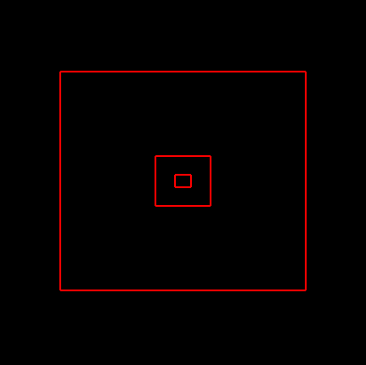
\includegraphics[scale=0.25]{images/anchors_3.png}
%    \caption{Anchors for the bus, car, and license plate classes}
%     \label{3_anchors}
%    \end{figure} 
    
    
    %We have tried to use three, four and five centroids, or clusters, in order to generate the anchors, but in all cases the outer boxes are the same and in the case of four and five anchors, only smaller and smaller anchors are added which are not different enough from each other, therefore we choose to use the variant with three anchors.% represented in Fig. \ref{3_anchors}. 
    
            
   \begin{figure}[!t]
      \centering
      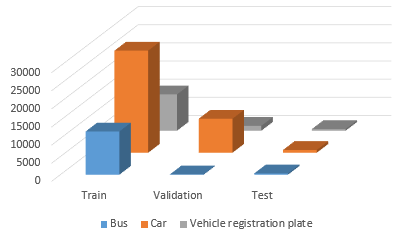
\includegraphics[scale=0.5]{images/enhanced_dataset.png}
      \caption{Undersampled and enhanced dataset bounding boxes distribution}
      \label{enhanced_distribution}
    \end{figure} 
    
    Each image needs to be associated with a ground truth. We represent the ground truth as a $C \times C \times B \times (5+N)$ tensor. For each cell in the $C \times C$ grid, we associate B anchor boxes. Each anchor box has the following parameters: $b_x$ and $b_y$ represent the center of the box, $b_w$ and $b_h$ represent the width and height, c is the probability that the anchor predicts an object and $c_1, c_2, c_3, ... c_n$ represent the class probabilities. In our case, C is 13 and both B and N are 3. Therefore, the output is a tensor of shape $13 \times 13 \times 3 \times 8$.
    
    The formulas that are used to compute the center, width, and height from the output of the model are:
    
    \begin{equation}
    \begin{split}
        & b_x = \sigma(t_x) + c_x \\
        & b_y = \sigma(t_y) + c_y \\
        & b_w = p_w \cdot e^{t_w} \\ 
        & b_h = p_h \cdot e^{t_h}
    \end{split}
    \label{conversion_formulas}
    \end{equation}
    
    Where $t_x, t_y, t_w, t_h$ represent the raw predictions to which the sigmoid function is applied, $c_x, c_y$ represent the coordinates of the upper left corner of the cell that predicts the box, and $p_w, p_h$ represent the width and height of the anchor that predicts the box. Over the output for the class probabilities, the softmax function is applied.
    
    
    
    \subsection{Model}
    The object detection model is inspired by YOLOv2 \cite{yolov2}. The neural network is fully convolutional and is composed of three parts: feature extractor, neck, and head. For the feature extractor, we use MobileNetv2 \cite{mobilenetv2} because of its flexibility and the fact that it uses depthwise convolutions, inverted residual blocks, and linear bottlenecks, which all help with performance, thus consuming less power, which is crucial for mobile solutions. Also, we use pretrained weights on ImageNet \cite{imagenet} to benefit from transfer learning.
    
    For the rest of the model, we use convolution blocks which are composed of a convolution layer that uses HeNormal initialization, batch normalization, and optionally LeakyReLU activation function. In general, we choose an alpha of 0.1 for LeakyReLU.
    
    The neck is inspired by U-Net \cite{unet}. The aim is to add features from earlier layers to the result through skip layers and upsample blocks that use transposed convolutions, followed by LeakyReLu and batch normalization. This helps the network to "see" the image at multiple resolutions as explained in the fine-grained features section in \cite{yolov2}.

    On top of the upsamlple blocks, a dropout layer is used for regularization in order to reduce overfitting. Another reason for adding this layer at this specific position is that the upsample blocks have the most trainable parameters, compared to other areas of the model. After the dropout layer, a convolutional block and two inverted residual blocks are added, which help in refining the feature maps.

    The head is composed of a convolution layer that has 24 filters in our case, so the final output is $13 \times 13 \times 3 \times 8$ after a reshape layer. This is because we use three anchors and three classes. This can vary if other datasets are used.
    
    Also, an additional input that represents all the true bounding boxes is directly added to the output. This is an implementation trick that only helps in the computation of the loss because, even though each image is associated with a specific anchor, it is not restricted to be predicted only by that anchor. If the IOU threshold between the predicted box from another anchor and one of the true bounding boxes is high enough, that prediction is considered correct. During normal inference, a dummy array is passed for this input.
    
    In total, our model has around 2 million parameters, out of which around 1.3 million are from MobileNet.
 
    


    \subsection{Loss}
    During training, we optimize a composed loss function adapted from \cite{experincor}: 
    
   \begin{equation*}
        L = L_{loc} + L_{obj} + L_{class}
        \label{total_loss}
    \end{equation*}
    
    The first component is basically a sum-squared error, handling the localization loss: 
    
    \begin{equation*}
    \begin{split}
        & L_{loc} = \frac{\lambda_{coord}}{N_{L^{obj}}}
        \sum_{i=0}^{S^2}\sum_{j=0}^B 
        L_{ij}^{obj} 
         \cdot [(x_{ij}-\hat{x}_{ij})^2 + 
        (y_{ij}-\hat{y}_{ij})^2 +\\
        & + (\sqrt{w_{ij}}-\sqrt{\hat{w}_{ij}})^2 + (\sqrt{h_{ij}}-\sqrt{\hat{h}_{ij}})^2 ]
    \end{split}
    \end{equation*}
    
    Where $
    L_{ij}^{obj} = \left\{
        \begin{array}{ll}
              1 & C_{ij} = 1\\
              0 & otherwise\\
        \end{array} 
        \right. 
    $ is an indicator function in which $C_{ij}$ means that there is an actual object in the i'th cell and j'th anchor. $N_{L^{obj}}$ just represents the number of actual object in the image and it is given by the following formula: $\sum_{i=0}^{S^2}\sum_{j=0}^B L_{ij}^{obj}$. The center of the bounding box is denoted using the $x$ for the horizontal position and $y$ for the vertical position. The width is denoted with $w$ and the height with $h$. The square root of the width and height is used because, otherwise, the error in small and large bounding boxes is treated the same.
    
    The second component is related to the objectness of a bounding box, which represents the probability that an object is present in that bounding box:
    
    \begin{equation*}
    \begin{split}
        & L_{obj} = \frac{\lambda_{obj}}{N^{conf}}
        \sum_{i=0}^{S^2}\sum_{j=0}^B
        L_{ij}^{obj}(IOU_{prediction_{i,j}}^{ground\;truth_{i,j}} - \hat{C}_{ij})^2 +\\
        & +\frac{\lambda_{noobj}}{N^{conf}}
        \sum_{i=0}^{S^2}\sum_{j=0}^B
        L_{ij}^{noobj}(0 - \hat{C}_{ij})^2
    \end{split}
    \end{equation*}
        
    Where \\ $
    L_{ij}^{noobj} = \left\{
        \begin{array}{ll}
              1 & max_{i'j'} IOU_{pred_{i,j}}^{GT_{i',j'}} < IOU_{t} \; and \; C_{ij} = 0\\
              0 & otherwise\\
        \end{array} 
        \right.
        $ is an indicator function which is one only if a predicted bounding box that does not appear in the ground truth in the respective cell and anchor, has the IOU overlap with any ground truth bounding box less than $IOU_{t}$. Basically, if the prediction has an IOU overlap with any bounding box larger than $IOU_{t}$, but it does not appear in the ground truth, then it is considered correct and it's not penalized, otherwise, it is not considered an object and it must increase the loss. Here we use the extra output explained in the previous section. $N^{conf} = \sum_{i=0}^{S^2}\sum_{j=0}^B L_{ij}^{obj} + L_{ij}^{noobj}(1-L_{ij}^{obj})$ counts the number of bounding boxes from the ground truth, but also the boxes that predict objects where there shouldn't be any. Therefore, the first part penalizes the errors in the confidence scores for objects that should be predicted, and the second part penalizes the boxes that predict an object that should not be there.
        
        
    
        
    The last component represents the loss from the class probabilities, and when multiple classes are involved, usually cross-entropy loss is used:
    
    \begin{equation*}
        L_{class} = - \frac{\lambda_{class}}{N_{L^{obj}}} 
        \sum_{i=0}^{S^2} \sum_{j=0}^B
        L_{ij}^{obj}
        \sum_{c \in classes}p_{ij}^c log(\hat{p}_{ij}^c)
        \label{class_loss}
    \end{equation*}
    
    
    
    Most grid cells do not contain any boxes. Therefore, in order to balance the confidence scores, $\lambda_{coord}=5$ and $\lambda_{noobj}=0.5$ are added in order to increase the loss from bounding box predictions and decrease the loss from confidence predictions. Also, $\lambda_{obj}=2$ and $\lambda_{class}=3$ are added to control the loss from the objectness and class losses. For $IOU_t$ we choose a value of 60\%.%In Table \ref{loss_hyperparameters}, we detail the values for these hyperparameters. 
    
    %\begin{table}[h]
    %\centering
    %\caption{Loss %hyperparameters}
    %\begin{tabular}{l|l}
    %$\lambda_{coord}$ & 5  % \\ \hline
    %$\lambda_{obj}$   & 2  % \\ \hline
    %$\lambda_{noobj}$ & 0.5 %\\ \hline
    %$\lambda_{class}$ & 3  % \\ \hline
    %IOU threshold     & 0.6
    %\end{tabular}
    %\label{loss_hyperparame%ters}
    %\end{table}
    

    \subsection{Data augmentation}
    
    We apply various photometric data augmentation techniques such as random hue (Fig. \ref{hue}), random brightness (Fig. \ref{brightness}), random contrast (Fig. \ref{contrast}) and random saturation (Fig. \ref{saturation}). The data augmentation techniques in Fig. \ref{photometric_data_augmentation} are applied over Fig. \ref{original}. 
    
    \def \scalevaraugmentation {0.09}
    \begin{figure}[!b] 
    \centering
    \subfloat[Original]{%
        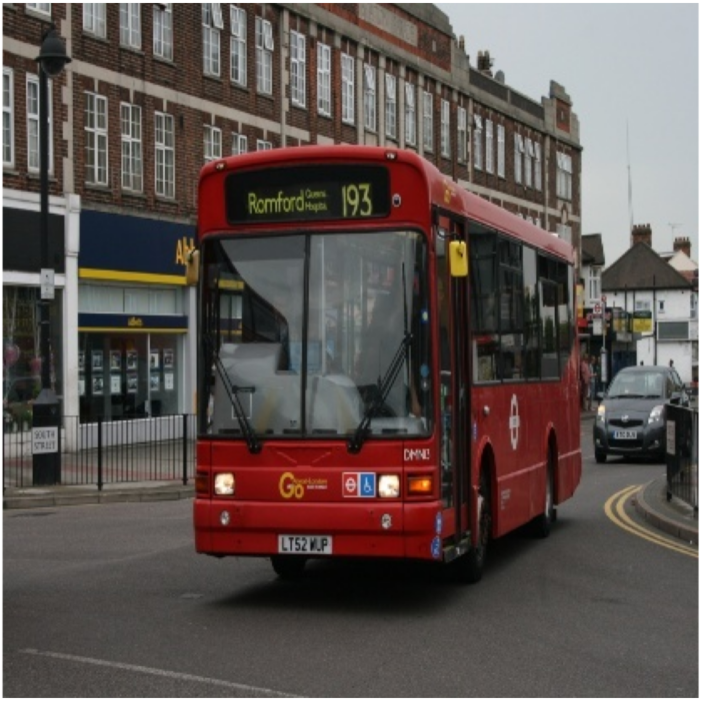
\includegraphics[scale=\scalevaraugmentation]{images/original.png}%
        \label{original}%
        }%
    \hfill%
    \subfloat[Hue]{%
        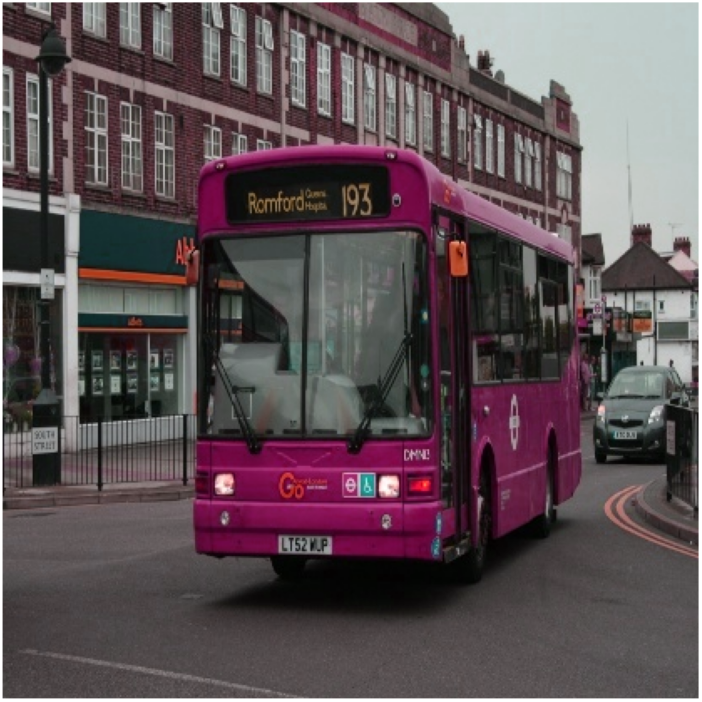
\includegraphics[scale=\scalevaraugmentation]{images/hue.png}%
        \label{hue}%
        }%
    \hfill%
    \subfloat[Brightness]{%
        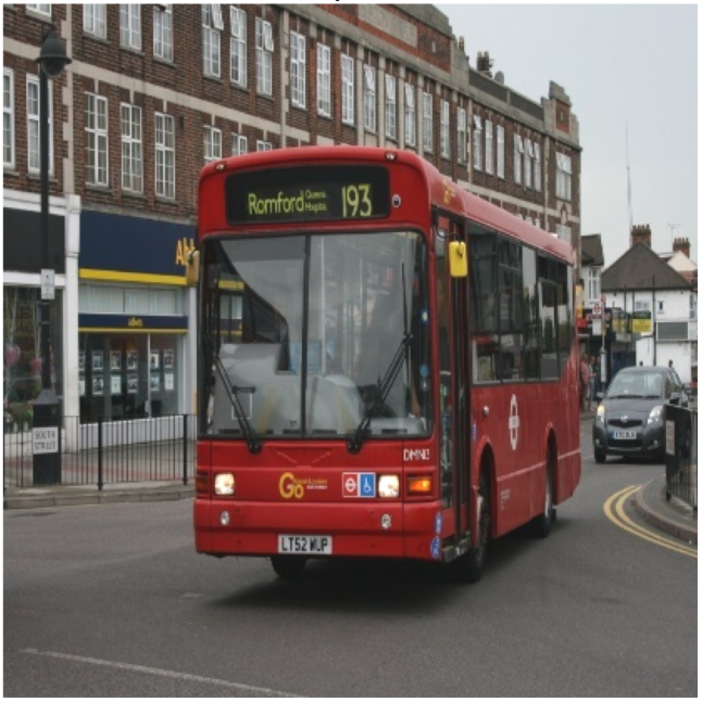
\includegraphics[scale=\scalevaraugmentation]{images/brightness.png}%
        \label{brightness}%
        }%
    \hfill%
    \subfloat[Contrast]{%
        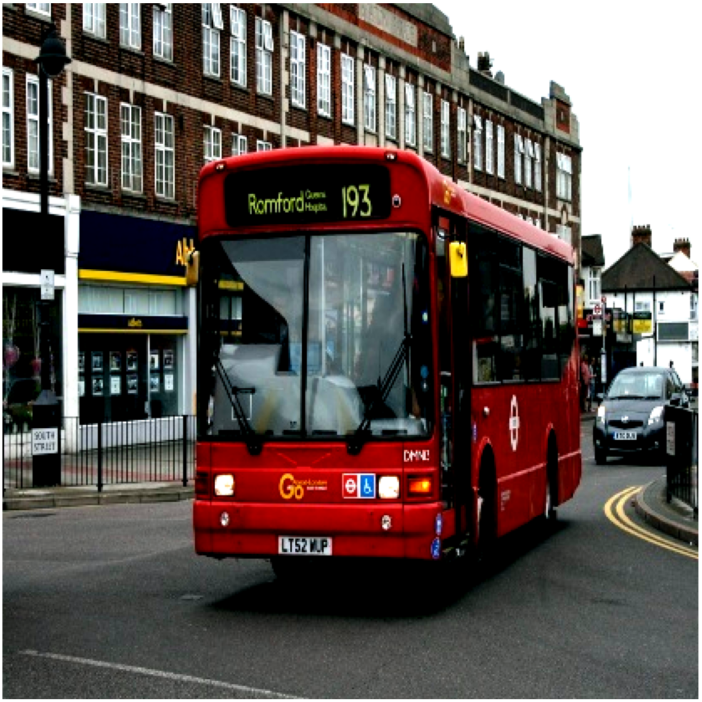
\includegraphics[scale=\scalevaraugmentation]{images/contrast.png}%
        \label{contrast}%
        }%
    \hfill%
    \subfloat[Saturation]{%
        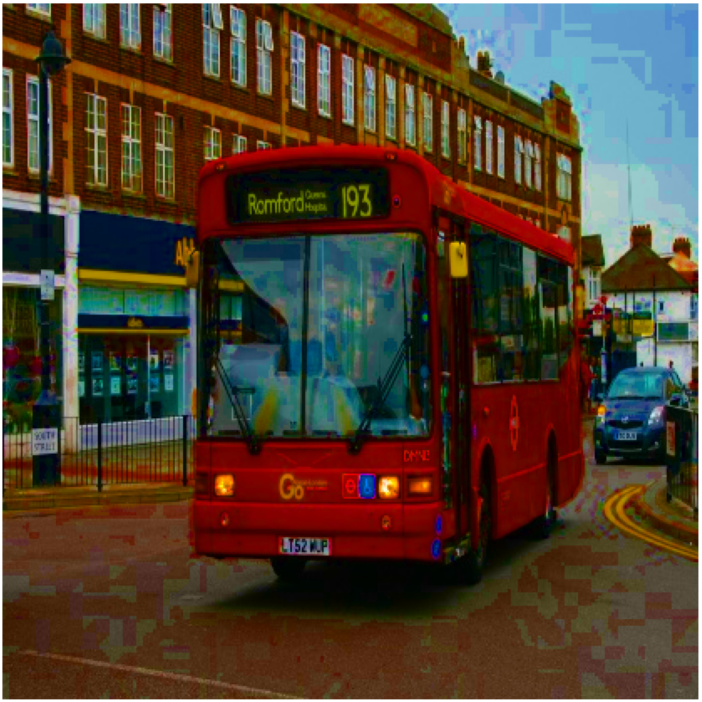
\includegraphics[scale=\scalevaraugmentation]{images/saturation.png}%
        \label{saturation}%
        }%
    \caption{Photometric data augmentation techniques}
    \label{photometric_data_augmentation}
    \end{figure}


    \def \scalevaraugmentationmosaic {0.12}
    \begin{figure}[t] 
    \centering
    \subfloat[Cutout]{%
        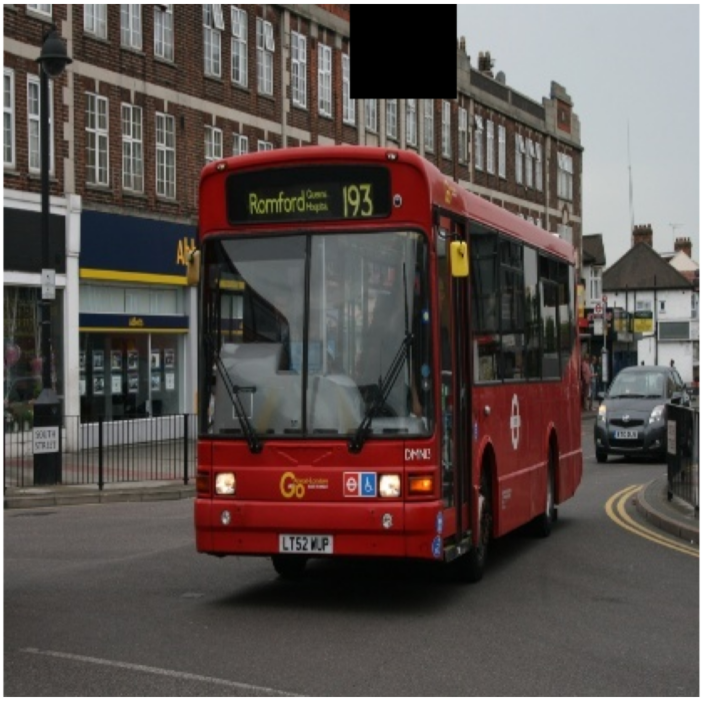
\includegraphics[scale=\scalevaraugmentationmosaic]{images/cutout.png}%
        \label{cutout}%
        }%
    \subfloat[Mosaic]{%
        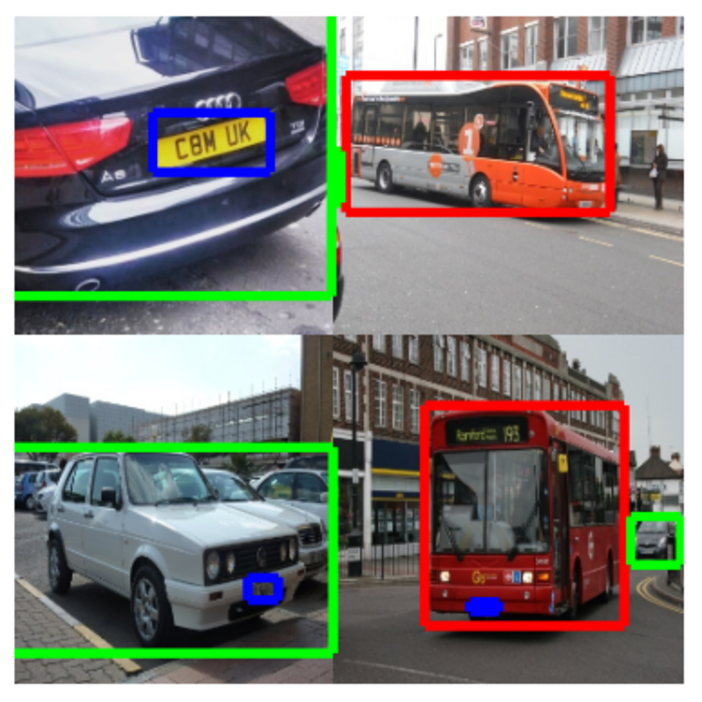
\includegraphics[scale=\scalevaraugmentationmosaic]{images/mosaic.png}%
        \label{mosaic}%
        }%
    \caption{Other data augmentation techniques}
    \label{other_data_augmentation}
    \end{figure}
    
    
    In Fig. \ref{other_data_augmentation} we present other data augmentation techniques that we have used. In Fig. \ref{cutout} we represent the Cutout technique, introduced in \cite{cutout}. The idea is to make the pixels from a random patch in the image black. This way the network should adapt to recognize objects even if they are partially visible. We also follow the recommendation from \cite{cutout}, which states that the patch doesn't have to fit fully in the image. This means that if the center of the patch falls near one of the edges of the image, only the part that overlaps with the images is blacked out.
    
    The other technique is called Mosaic, Fig. \ref{mosaic}, and it was first introduced in \cite{yolov4}. Here, four images are concatenated in order to form a single image. The effect is that the number of bounding boxes in a single image is increased, and the size of the bounding boxes becomes smaller, thus the network should better adapt to small bounding boxes. 

    
    In practice, for each image, we apply a random data augmentation technique from Fig. \ref{photometric_data_augmentation}, and we apply all these data augmentation techniques only during training, and all of them, except Mosaic, are vectorized in order to be computed on the GPU.



    \subsection{Training}
    
    For training, we use a pretrained version of MobileNetV2 \cite{mobilenetv2} on ImageNet \cite{imagenet}, and for the optimizer we use Adam. We use a cosine annealing scheduler for the learning rate, described in \cite{cosine_scheduler}, which follows the following formula:
    
    \begin{equation}
        LR_{epoch} = \eta_{min} + \frac{1}{2} (\eta_{max} - \eta_{min}) \cdot (1 + cos(\frac{epoch}{T} \cdot \pi))
        \label{cosine_formula}
    \end{equation}
    
    The main idea is that the learning rate will follow a cosine wave between $\eta_{min}$ and $\eta_{max}$. The epoch represents the current epoch, and $T$ represents the restart epoch, meaning that every $T$ epochs the monotony is changed, and the learning rate will reach either $\eta_{min}$ or $\eta_{max}$. %We can better see the phenomenon in Fig. \ref{scheduler}, where various schedules for the learning rate are plotted over a total of 50 epochs. We can see that when $T$ is equal to the total number of epochs, the learning rate decreases monotonously from the maximum to the minimum. If $T$ is larger than the number of epochs, then the learning rate doesn't even reach the minimum, and if the learning rate is smaller than the number of epochs, the cosine wave can be seen, and every $T$ epochs, the slope changes.
    
    %\begin{figure}[t]
    %    \centering
    %    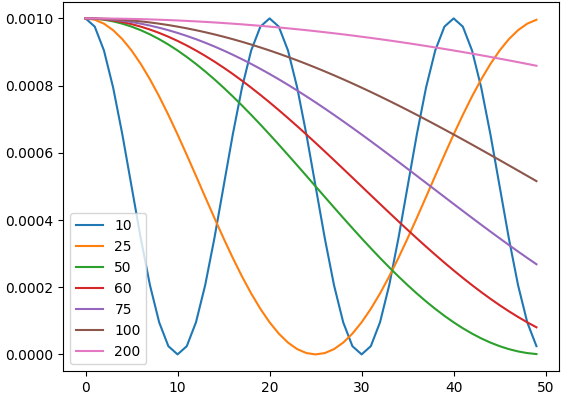
\includegraphics[scale=0.4]{images/scheduler.png}
    %    \caption{Cosine annealing scheduler}
    %    \label{scheduler}
    %\end{figure}
    
    
    
    We train the model for 50 epochs on a GPU using early stop with the patience of 5 epochs and a delta of $1e^{-4}$. This means that if the model does not improve after some epochs, by the given delta, the training stops because we don't want to overtrain, in order to both save time and reduce overfitting also.
    
    At the beginning of the epoch, the learning rate is set, following the cosine annealing formula, and at the end, the images are shuffled in order for the network to see the images in a different order, each epoch. Also, during training, before any processing, random photometric data augmentation is used, followed by cutout and mosaic as explained in a previous section.
    
    During a normal training session, the weights of the pretrained model are frozen, meaning that they do not update. We do this in order to not break the knowledge stored in the weights. But, during a fine tuning session, which occurs after a normal training session, we set a very small learning rate and unfreeze the pretrained model. By doing this, the previously frozen weights are updated to better fit our dataset. Usually, a fine tuning epoch takes much longer, because the pretrained model has the largest share in parameters of the total number of parameters.

     In Fig. \ref{model_v42_loss} we present the evolution of the loss during training for our best model. Ideally, the validation loss is always around the training loss. This is a sign that the model does not overfit.
     
     \begin{figure}[b]
        \centering
        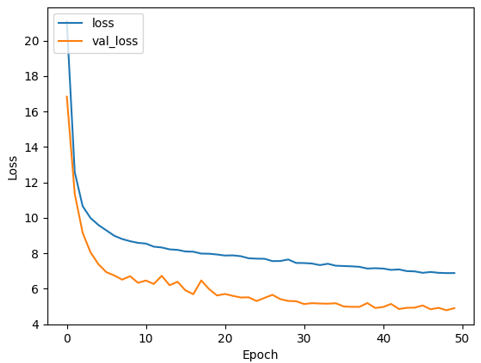
\includegraphics[scale=0.25]{images/model_v42_train.png}
        \caption{Training (blue) and validation (orange) loss for our best model}
        \label{model_v42_loss}
    \end{figure}
    \subsection{Inference}
    The inference represents a pipeline of processing an input and getting the predictions for that input. In our case, the input is an image and there are three stages of processing that an image goes through in order to get the output, represented by the bounding boxes.

   Firstly, there is preprocessing, which consists of normalizing the images in the range [-1, 1]. This is required by the MobileNetV2 backbone model. Also, here the data augmentation occurs, before the normalization.
   
   The second step is passing the image through the actual neural network.
    
    Postprocessing is the final step. Firstly, the bounding boxes are extracted from the resulting tensor of size $C \times C \times B \times (5+C)$. Basically, for each cell in the $C \times C$ grid, we extract the $B \cdot (5+C)$ raw bounding boxes. Then the raw values are converted using \ref{conversion_formulas} to obtain the actual values. These boxes are filtered based on their score.
    
    Usually, there are a lot of overlapping boxes that predict the same object. This is solved using Non-maximum Suppression (NMS) which prunes away extra bounding boxes by ordering the boxes by their scores, descending. Then each box is kept only if they have a low enough IOU with any previously kept bounding box with the same label. In this way, if there are a lot of boxes with the same label in some area, only the one with the highest score is kept. 
    
    %This stage introduces two new hyperparameters. One that controls the minimum score threshold of the bounding boxes, and one that controls the maximum IOU a bounding box can have with other boxes with the same label for NMS.
